\subsection{Module} \label{subsec:module}
De module is de Haskell bibliotheek die de programmeur gebruikt om de grafische interface in de client te bedienen. Naar de programmeur is de gebruiksvriendelijkheid van de bibliotheek een van de belangrijkste overwegingen voor het ontwerp. De module bestaat uit een aantal onderdelen: de server die de statische bestanden serveert, de WebSocket server die de verbinding met de client onderhoudt, en de laag die de input en output verwerkt. \autoref{fig:architecture_module} geeft de architectuur weer van de module.

\begin{figure}
\begin{center}
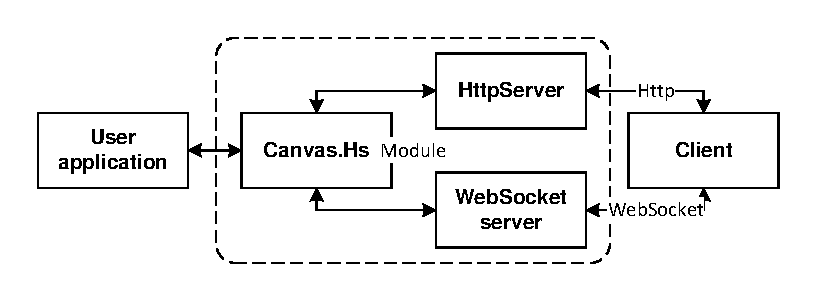
\includegraphics[keepaspectratio,width=\textwidth]{./images/module_architecture.pdf}
\caption{Architectuur van de module}
\label{fig:architecture_module}
\end{center}
\end{figure}

\paragraph{Servers}
Canvas.hs draait een simpele server op port 8000 die statische bestanden kan serveren. Waaronder de index pagina, de JavaScript bestanden en eventueel plaatjes. Op port 8080 draait een WebSocket server die de verbinding met de client onderhoudt.


\paragraph{Server in de module}
De server draait in het proces dat gestart wordt vanuit de Haskell-code van de programmeur. De main van de programmeur start (indirect) de server. Dit is eenvoudiger dan het draaien van de server in een apart proces. Er hoeft namelijk niet tussen verschillende Haskell-processen gecommuniceerd te worden. Dit scheelt het schrijven van nog een interface tussen het server- en het module proces. Nadeel is wel dat het voortdurend opnieuw starten en afsluiten van de server leidt tot vertraging in het opstarten van het programma van de programmeur. Dit is vervelend als de programmeur regelmatig kleine wijzigingen maakt en dan de code opnieuw moet starten. Echter lijkt de overhead van het opnieuw starten van de server minimaal. Het is verder praktisch dat er geen rekening gehouden hoeft te worden met de state van de server bij het opstarten van het programma.

\paragraph{Gebruik} Wanneer de programmeur gebruik wil maken van Canvas.hs moet hij gebruik maken van de installEventHandler functie. Bij het aanroepen van deze functie moet de programmeur een eventHandler meegeven die alle events vanuit de interface afhandelt. Om het gebruik van Canvas.hs zo makkelijk mogelijk te houden zal bij het aanroepen van installEventHandler automatisch de statische server en de WebSocket server gestart worden, en daarna automatisch de browserpagina geopend worden. \autoref{fig:startup_procedure} geeft de opstartprocedure weer.

\begin{figure}
\begin{center}
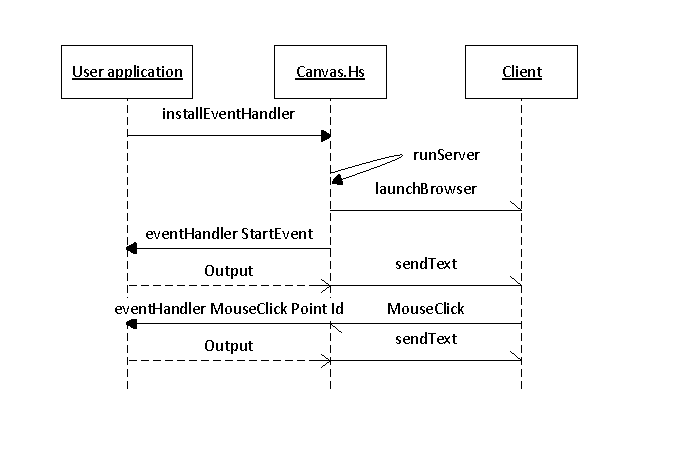
\includegraphics[keepaspectratio,width=\textwidth]{./images/module_startup_procedure_interaction.pdf}
\caption{De opstartprocedure en initiele interactiesequentie}
\label{fig:startup_procedure}
\end{center}
\end{figure}

\paragraph{Input/output}
De module handelt input en output af door events naar de eventHandler van de programmeur te sturen. Bijvoorbeeld: wanneer een gebruiker op een rondje klikt zal het programma de eventHandler aanroepen met de ID van dat rondje en de locatie van de muisklik. De eventHandler van de programmeur kan dan nieuwe output genereren op basis van dit event. Zoals een nieuw menu weergeven of het uitvoeren van een actie zoals het opvragen van een bestand van de gebruiker. In \autoref{fig:startup_procedure} is deze interactie weergegeven.

De programmeur zal in zijn eventHandler bij ieder event de huidige state en de huidige event meekrijgen. Het type van de eventhandler is \inlinecode{userState -> Event -> (userState, Output)}, waarin de programmeur elk type aan userState kan geven. Door middel van pattern matching kan de programmeur makkelijk een bepaald event opvangen. Bijvoorbeeld: een muisklikevent wordt opgevangen door: \inlinecode{handler state (MouseClick (x,y) "id")}. De returnwaarde van de eventhandler is een tuple van de nieuwe state en de output. Output is of \inlinecode{BlockingAction action} of een \inlinecode{Out (Maybe Shape, [Action])}, zo kan de gebruiker of een enkele blocking actie doen, of een shapen en een lijst van acties teruggeven. Voor een volledige lijst van (blocking-)acties kan \autoref{subsec:grafische_bibliotheek} bekeken worden.

\paragraph{Timers}
Canvas.hs ondersteunt timers die met een bepaald interval events naar de eventHandler sturen. Op deze manier is het mogelijk om bijvoorbeeld animaties of andere periodieke updates uit te voeren. Er is voor gekozen om de timers te laten draaien in de module, en niet in de JavaScript applicatie. Dit had voornamelijk als reden dat de JavaScript applicatie ontworpen is voor interactie met de cliënt en het laten lopen van timers daar niet onder valt. Daarnaast heeft het als bijkomend voordeel dat de timer events niet via de WebSocket verstuurd hoeven te worden.

\paragraph{Unsafe I/O}
In de HTTP- en WebSocketsserver wordt gebruik gemaakt van \inlinecode{unsafePreformIO} voor het bijhouden van een lijst van child processen (een MVar die threads bijhoudt) en voor het bijhouden van de verbinding met client (een IORef die de connection naar de client bevat). Hoewel het gebruik van \inlinecode{unsafePreformIO} in dit geval volkomen veilig is, zijn er bezwaren tegen het gebruik van ervan\cite{Haskell.org2008}. Dit is namelijk niet de netste oplossing en kan meestal voorkomen worden. Het is netter om m.b.v. bijvoorbeeld de StateT-monad de server deze zaken bij te laten houden. Echter is het implementeren daarvan tijdsintensief en is daarom voor deze oplossing gekozen.
